% Options for packages loaded elsewhere
\PassOptionsToPackage{unicode}{hyperref}
\PassOptionsToPackage{hyphens}{url}
%
\documentclass[
]{book}
\usepackage{amsmath,amssymb}
\usepackage{lmodern}
\usepackage{iftex}
\ifPDFTeX
  \usepackage[T1]{fontenc}
  \usepackage[utf8]{inputenc}
  \usepackage{textcomp} % provide euro and other symbols
\else % if luatex or xetex
  \usepackage{unicode-math}
  \defaultfontfeatures{Scale=MatchLowercase}
  \defaultfontfeatures[\rmfamily]{Ligatures=TeX,Scale=1}
\fi
% Use upquote if available, for straight quotes in verbatim environments
\IfFileExists{upquote.sty}{\usepackage{upquote}}{}
\IfFileExists{microtype.sty}{% use microtype if available
  \usepackage[]{microtype}
  \UseMicrotypeSet[protrusion]{basicmath} % disable protrusion for tt fonts
}{}
\makeatletter
\@ifundefined{KOMAClassName}{% if non-KOMA class
  \IfFileExists{parskip.sty}{%
    \usepackage{parskip}
  }{% else
    \setlength{\parindent}{0pt}
    \setlength{\parskip}{6pt plus 2pt minus 1pt}}
}{% if KOMA class
  \KOMAoptions{parskip=half}}
\makeatother
\usepackage{xcolor}
\usepackage{longtable,booktabs,array}
\usepackage{calc} % for calculating minipage widths
% Correct order of tables after \paragraph or \subparagraph
\usepackage{etoolbox}
\makeatletter
\patchcmd\longtable{\par}{\if@noskipsec\mbox{}\fi\par}{}{}
\makeatother
% Allow footnotes in longtable head/foot
\IfFileExists{footnotehyper.sty}{\usepackage{footnotehyper}}{\usepackage{footnote}}
\makesavenoteenv{longtable}
\usepackage{graphicx}
\makeatletter
\def\maxwidth{\ifdim\Gin@nat@width>\linewidth\linewidth\else\Gin@nat@width\fi}
\def\maxheight{\ifdim\Gin@nat@height>\textheight\textheight\else\Gin@nat@height\fi}
\makeatother
% Scale images if necessary, so that they will not overflow the page
% margins by default, and it is still possible to overwrite the defaults
% using explicit options in \includegraphics[width, height, ...]{}
\setkeys{Gin}{width=\maxwidth,height=\maxheight,keepaspectratio}
% Set default figure placement to htbp
\makeatletter
\def\fps@figure{htbp}
\makeatother
\setlength{\emergencystretch}{3em} % prevent overfull lines
\providecommand{\tightlist}{%
  \setlength{\itemsep}{0pt}\setlength{\parskip}{0pt}}
\setcounter{secnumdepth}{5}
\usepackage{booktabs}
\usepackage{amsthm}
\makeatletter
\def\thm@space@setup{%
  \thm@preskip=8pt plus 2pt minus 4pt
  \thm@postskip=\thm@preskip
}
\makeatother

\usepackage{tcolorbox}
\tcbuselibrary{breakable}

\newtcolorbox{blackbox}{
  colback=black,
  coltext=white,
  colframe=black,
  boxsep=5pt,
  arc=4pt,
  breakable
  }
\newtcolorbox{bonus}{
  colback=blue!15,
  colframe=blue!15,
  coltext=black!80,
  boxsep=5pt,
  arc=4pt,
  breakable
  }
\newtcolorbox{reflect}{
  colback=green!5,
  colframe=green!5,
  coltext=black!80,
  boxsep=5pt,
  arc=4pt,
  breakable
  }
\newtcolorbox{assessment}{
  colback=blue!5,
  colframe=blue!5,
  coltext=black!80,
  boxsep=5pt,
  arc=4pt,
  breakable
  }
  
\newtcolorbox{progress}{
  colback=purple!10,
  colframe=purple!10,
  coltext=black!80,
  boxsep=5pt,
  arc=4pt,
  breakable
  }
\newtcolorbox{video}{
  colback=yellow!5,
  colframe=yellow!5,
  coltext=black!80,
  boxsep=5pt,
  arc=4pt,
  breakable
  }
\newtcolorbox{caution}{
  colback=red!5,
  colframe=red!5,
  coltext=black!80,
  boxsep=5pt,
  arc=4pt,
  breakable
  }
\newtcolorbox{feedback}{
  colback=black!5,
  colframe=black!5,
  coltext=black!80,
  boxsep=5pt,
  arc=4pt,
  breakable
  }
\ifLuaTeX
  \usepackage{selnolig}  % disable illegal ligatures
\fi
\usepackage[]{natbib}
\bibliographystyle{apalike}
\IfFileExists{bookmark.sty}{\usepackage{bookmark}}{\usepackage{hyperref}}
\IfFileExists{xurl.sty}{\usepackage{xurl}}{} % add URL line breaks if available
\urlstyle{same} % disable monospaced font for URLs
\hypersetup{
  pdftitle={{[}Course Name \& \#{]}},
  pdfauthor={Name},
  hidelinks,
  pdfcreator={LaTeX via pandoc}}

\title{{[}Course Name \& \#{]}}
\author{Name}
\date{}

\begin{document}
\maketitle

{
\setcounter{tocdepth}{1}
\tableofcontents
}
\hypertarget{welcome}{%
\chapter*{Welcome}\label{welcome}}
\addcontentsline{toc}{chapter}{Welcome}

\emph{Insert the course description here.}

\begin{feedback}
\textbf{Tips for Instructors:}
Consider this description as a hook to get students interested in your course. Describe the big ideas of your course, summarize what students will learn, explain why it matters.
\textbf{\emph{Note that if there are any changes to a course description, these need to be approved by Senate.}}
\end{feedback}

\hypertarget{how-to-navigate-this-book}{%
\subsection*{How To Navigate This Book}\label{how-to-navigate-this-book}}
\addcontentsline{toc}{subsection}{How To Navigate This Book}

To move quickly to different portions of the book, click on the appropriate chapter or section in the table of contents on the left. The buttons at the top of the page allow you to show/hide the table of contents, search the book, change font settings, download a pdf or ebook copy of this book, or get hints on various sections of the book.

\includegraphics{assets/course-intro/menu.png}

The faint left and right arrows at the sides of each page (or bottom of the page if it's narrow enough) allow you to step to the next/previous section. Here's what they look like:

\includegraphics{assets/course-intro/left_arrow.png} 
\includegraphics{assets/course-intro/right_arrow.png}

You can also download an offline copy of this books in various formats, such as pdf or an ebook. If you are having any accessibility or navigation issues with this book, please reach out to your instructor or our online team at \href{mailto:elearning@twu.ca}{\nolinkurl{elearning@twu.ca}}

\hypertarget{course-units}{%
\subsection*{Course Units}\label{course-units}}
\addcontentsline{toc}{subsection}{Course Units}

This course is organized into 10 units. Each unit of the course will provide you with the following information:

\begin{itemize}
\tightlist
\item
  A general overview of the key concepts that will be addressed during the unit.\\
\item
  Specific learning outcomes and topics for the unit.\\
\item
  Learning activities to help you engage with the concepts. These often include key readings, videos, and reflective prompts.\\
\item
  The Assessment section provides details on assignments you will need to complete throughout the course to demonstrate your understanding of the course learning outcomes.
\end{itemize}

\begin{caution}
Note that assessments, including assignments and discussion posts will be submitted in Moodle. See the Assessment tab in Moodle for the assignment dropboxes.
\end{caution}

\hypertarget{course-activities}{%
\subsection*{Course Activities}\label{course-activities}}
\addcontentsline{toc}{subsection}{Course Activities}

Below is some key information on features you will see throughout the course.~

\begin{reflect}
\textbf{\emph{Learning Activity}}\\
This box will prompt you to engage in course concepts, often by viewing resources and reflecting on your experience and/or learning. Most learning activities are ungraded and are designed to help prepare you for the assessment in this course.
\end{reflect}

\begin{assessment}
\textbf{\emph{Assessment}}\\
This box will signify an assignment or discussion post you will submit in Moodle. Note that these demonstrate your understanding of the course learning outcomes. Be sure to review the grading rubrics for each assignment.
\end{assessment}

\begin{progress}
\textbf{\emph{Checking Your Learning}}\\
This box is for checking your understanding, to make sure you are ready for what follows.
\end{progress}

\begin{feedback}
\textbf{\emph{Note}}\\
This box signifies Tips for Instructors. Please delete these before you share this course book with your students!
\end{feedback}

\hypertarget{the-nature-of-moral-inquiry}{%
\chapter{The Nature of Moral Inquiry}\label{the-nature-of-moral-inquiry}}


\includegraphics{assets/unit_1/U1_baby-2709666_1920.jpg}

\emph{Picture of a child infront of a laptop. Photo Credit: \href{https://pixabay.com/en/baby-learn-laptop-question-2709666/}{Pixabay}}

\hypertarget{overview}{%
\section*{Overview}\label{overview}}
\addcontentsline{toc}{section}{Overview}

Welcome to Unit 1 of \emph{Ethical Issues}, Philosophy 210. When was the last time you had a free and open discussion with a group of friends about the issues of abortion, world hunger, animal rights, sexual morality, capital punishment, war and peace, or proper treatment of the environment? We often tend to avoid topics like these to keep the peace in polite company.

You may have noticed that people often get very passionate, even angry, over moral issues like the ones mentioned above, and this can lead to highly emotional discussions which often shed more heat than light on the issues.

The word, ``ethics,'' comes from a Greek word \emph{ethos} which meant custom or habit. Ethics is a branch of philosophy which is concerned with questions of right and wrong, good and evil. As such it addresses a number of sensitive moral issues, the kind some of us may try to avoid in day-to-day conversation.

Are there ways we can think through and engage such issues in a cool and enlightening manner? Are there steps or procedures that can guide us to thoughtful conclusions? Here is where the discipline of ethics can come in. As a discipline, ethics is devoted to identifying hard moral questions on which people disagree and then applying relevant moral principles to these questions in the search for correct moral action. As such, it can provide a better way of thinking through these issues and for this reason, ethics is a highly practical and useful discipline.

In some cases, people who heatedly disagree about a moral question may find that they actually agree on the guiding moral principles but just differ on how these principles are to be applied. In other words, the parts they agree on are larger than those on which they disagree. That can allow for a cooler and more productive discussion of sensitive moral questions and can even point the way for them to come to a solution.

In this unit we will turn our attention to a number of foundational concepts involved in moral reasoning. Our goal will be to develop a moral outlook, to learn to think ethically about the moral questions we face in life.

One of the first things to remember is that ethics is different from most other disciplines in a highly significant way. While most other areas of study such as science, history, and mathematics are descriptive, ethics is prescriptive. Ethical judgments actually prescribe certain behaviours. They tell us we ought to do certain things, or refrain from them. In fact, words like right, wrong, should, ought, and even deserve, are key indicators in any sentence that we may be making ethical judgments about something.

If your friend described the medical service she just received as slow or unhelpful, she would have made a purely descriptive statement. If, however, she followed it up by saying the government ought to be providing faster and more effective health care, she would have made a moral judgment. She would have prescribed one type of behaviour and said the government ought to have acted that way. In other words, she has now moved into the moral realm; she is involved in moral discourse.

In this unit we will explore further how to carry out moral discourse well and will examine the interesting question of why, around the world, people do not always appear to have the same moral outlook.

\hypertarget{topics}{%
\subsection*{Topics}\label{topics}}
\addcontentsline{toc}{subsection}{Topics}

This unit is divided into 3 topics:

\begin{enumerate}
\def\labelenumi{\arabic{enumi}.}
\tightlist
\item
  Developing a Moral Outlook
\item
  Moral Reasoning
\item
  Cultural Relativism
\end{enumerate}

\hypertarget{learning-outcomes}{%
\subsection*{Learning Outcomes}\label{learning-outcomes}}
\addcontentsline{toc}{subsection}{Learning Outcomes}

When you have completed this unit, you should be able to:
- Define key terms, such as meta-ethics, normative ethics, applied ethics, and moral intuition.
- Describe what it means to think ethically about key moral dilemmas we face in the 21st century.
- Explain some unique features of moral discourse.
- Discuss how cultural relativism differs from moral objectivism.
- Take a position on the issue of cultural relativism, however tentatively, and articulate both the strongest arguments for and some key objections to it.

\hypertarget{activity-checklist}{%
\subsection*{Activity Checklist}\label{activity-checklist}}
\addcontentsline{toc}{subsection}{Activity Checklist}

Here is a checklist of learning activities you will benefit from in completing this unit. You may find it useful for planning your work.

\begin{reflect}
\hypertarget{learning-activities}{%
\subsubsection*{Learning Activities}\label{learning-activities}}
\addcontentsline{toc}{subsubsection}{Learning Activities}

\textbf{Introductions} : Introduce yourself to your peers.

\textbf{Read, View, Reflect} :

Read pages 1-7 of the \emph{An Introduction to Moral Philosophy} by Jonathan Wolff. Watch the videos related to the topic.

Read the rest of Chapter 1 (pages 7-17) of your textbook, \emph{An Introduction to Moral Philosophy}. Watch the videos related to the topic.

Read chapter 2 of your \emph{Introduction} textbook. Watch the videos related to the topic.

\textbf{Thought Experiment} :

Read and analyze the thought experiment on page 14 of the Wolff text.

\textbf{Key Terms Quiz} :

Take the ungraded quiz to review important concepts.

\hypertarget{assignment}{%
\subsubsection{\texorpdfstring{\textbf{Assignment} :}{Assignment :}}\label{assignment}}

Ethics Committee Response (15\%)
\end{reflect}

\hypertarget{resources}{%
\subsection*{Resources}\label{resources}}
\addcontentsline{toc}{subsection}{Resources}

Here are the resources you will need to complete this unit.
- Wolff, Jonathan. ~\emph{An Introduction to Moral Philosophy}. ~New York: W. W. Norton \& Company, 2018. ~
- Other online resources will be provided in the unit.

\begin{reflect}
\hypertarget{activity-introductions}{%
\subsection*{Activity : Introductions}\label{activity-introductions}}
\addcontentsline{toc}{subsection}{Activity : Introductions}

Before you delve into the course material, take some time to introduce yourself to your peers, your facilitator, and your instructor. Share a bit about yourself, such as where you live, what you are studying, the kind of things that interest you, and perhaps some questions you have about this course. Feel free to share a picture of something that means something to you (e.g.~pet, family, favourite book, etc.).
Note that in this course, you will write reflective journals and participate in other group assignments. This is a good opportunity to get to know each other and build your community of learners.

Go to the Course Cafe section and click on Student Introductions. Add your introduction to the forum.
\end{reflect}

\hypertarget{developing-a-moral-outlook}{%
\section*{Developing a Moral Outlook}\label{developing-a-moral-outlook}}
\addcontentsline{toc}{section}{Developing a Moral Outlook}

Moral ideas and teachings are not really new to any of us, whether we have ever taken a course in ethics or not. We have all been taught from our earliest days to obey our parents, respect our elders, be kind to children, and a host of other moral instructions. In other words, ethics have been part of our lives from the beginning.

The process of developing a moral outlook begins by considering whether moral questions matter and, if they do, how we can develop attitudes that are sensitive to them. Does it matter whether I live one way or another, whether I help people or hurt them, lie to my neighbours or tell them the truth, respect other people's property or take it at will so long as I can get away with it?

When someone tells you that stealing your colleague's wallet was wrong and you reply by asking, ``Why should I care about that?'' you have commented on the necessity, or lack thereof, of a moral outlook.

One key area of study involved in developing a moral outlook is \textbf{meta-ethics,} which involves foundational questions of the nature of morality, how we know moral rules, etc. Another is \textbf{normative ethics} which is the study of what we are morally obligated to do. A third is \textbf{applied ethics} which moves one into the analysis of specific moral questions. In this topic, it will be important to understand the differences between these terms.

\begin{reflect}
\hypertarget{activity-read-view-and-reflect}{%
\subsection*{Activity : Read, View and Reflect}\label{activity-read-view-and-reflect}}
\addcontentsline{toc}{subsection}{Activity : Read, View and Reflect}

In the first activity, you are asked to read pages 1-7 of your textbook, \emph{An Introduction to Moral Philosophy} by Jonathan Wolff. As you read, be sure to take notes in your Learning Journal, defining key terms and explaining key concepts. Study the chapter review summary, questions and key terms. This will help you as you complete the assessments in this course.
Next, watch the following videos to learn more about the key terms from this section.

//todo \#1
\end{reflect}

\begin{caution}
\emph{Note that the learning activities in this course are ungraded, unless specified. You are strongly encouraged to complete them, as they are designed to help you succeed in your course assessments.}
\end{caution}

\hypertarget{moral-reasoning}{%
\section*{Moral Reasoning}\label{moral-reasoning}}
\addcontentsline{toc}{section}{Moral Reasoning}

What is moral reasoning or moral discourse? We are involved in moral reasoning
when we engage in a thinking process about what we ought to do in specific
situations. This will mean following a thoughtful procedure for sorting through
moral questions with the goal of discovering correct moral action. But how does
one do this?

One suggested method is the following:

\textbf{Step one}: Identify the precise foundational moral question needing to be resolved. For example, in the debate over the moral permissibility of abortion on demand, the foundational moral question concerns the nature and moral status of the unborn human being. Does it have the same status or value as a 3-year old child or that of a growth which needs to be removed? If this question were resolved and agreed upon by most people, there would be little left to argue about on this question. Admittedly, this is a difficult question but that is often the case in ethics. It's why we call them moral dilemmas. The point of identifying the key foundational question/s for each issue is that, then, at least we are thinking about the right questions and not wasting our time on others.

\textbf{Step two}: State the main answers to this question. This will involve accurately stating the main competing views on this moral question, both the ones we agree with and the ones we do not.

\textbf{Step three}: Discover the best arguments or reasons given for each of these answers. The goal is to understand the supporting rationale for each of these positions as well as the people who believe them.

\textbf{Step four}: Evaluate and assess these arguments with the goal of drawing a conclusion of your own concerning which answer is the best one. Normally the way to do step four well is to have done step three carefully. Reading the arguments for one view provides the most helpful material needed to evaluate both it and the opposing views.

In the end, you will find that proper moral reasoning involves applying general
moral principles such as the principles of love, justice, human dignity,
honesty, etc., to specific moral questions in order to see what these principles
tell us about the correct course of action.

Of course, moral reasoning needs to be done with great care. In the text reading
for this topic, we will learn a few principles for careful reasoning. One
important concept in the reading is \textbf{logical validity} which occurs when the
conclusion of an argument follows logically from the premises. This means that
if the premises are true, the conclusion must also be true. If an argument,
moral or otherwise, is invalid (i.e., if the conclusion does not follow from the
premises), it proves nothing and should be set aside.

Some other terms are \textbf{argument by analogy}, \textbf{argument to the best
explanation, moral intuitions, universalization} and the \textbf{fact/value
distinction.} Our text will explain them and we will have an opportunity to
think through their importance for careful reasoning with our class colleagues.

\begin{reflect}
\hypertarget{learning-activities-1}{%
\subsection*{Learning Activities}\label{learning-activities-1}}
\addcontentsline{toc}{subsection}{Learning Activities}

\hypertarget{read-view-and-reflect}{%
\subsubsection*{Read, View and Reflect}\label{read-view-and-reflect}}
\addcontentsline{toc}{subsubsection}{Read, View and Reflect}

Read the rest of Chapter 1 (pages 7-17) of your textbook, \emph{An Introduction to
Moral Philosophy} by Jonathan Wolff. Take notes on key terms and concepts.

Next, watch the following videos to get a better understanding of key terms for
this topic.

\hypertarget{thought-experiment}{%
\subsubsection*{Thought Experiment}\label{thought-experiment}}
\addcontentsline{toc}{subsubsection}{Thought Experiment}

Read the thought experiment posed by philosopher, Philippa Foot, on page 14 of the Wolff text, \emph{Introduction to Moral Philosophy}. Consider how you might answer the question posed by this thought experiment and why you would answer this way. What ethical issues arise?
\end{reflect}

\begin{caution}
\emph{Note that this is an ungraded activity, but you are encouraged to write your answers in your notes. You may be asked to review this case or similar cases in your class discussion groups. This practice of analyzing a case, contemplating various perspectives, and presenting an argument will help you in your assessments for this course.}
\end{caution}

\hypertarget{cultural-relativism}{%
\section*{Cultural Relativism}\label{cultural-relativism}}
\addcontentsline{toc}{section}{Cultural Relativism}

This topic will introduce us to one of the most perplexing questions about
morality: are moral values consistent for all people regardless of when or where
they happen to live? If so why do moral values seem to vary, sometimes
considerably, in different times and cultures?

\textbf{Cultural Relativism} is more than the recognition that moral views and
practices differ from place to place and time to time. It is the view that what
is morally right and wrong should be understood only within a specific cultural
or social setting. Furthermore, what is morally right in one culture may be
wrong in another. In other words it is a view about the very nature of morality.

In chapter 2 of the Wolff \emph{Introduction} text, we will come across a number of
different kinds of relativism and will have the opportunity to learn some
arguments often made in favour of cultural relativism along with a number of
serious problems with it.

\hypertarget{learning-activities-2}{%
\subsection*{Learning Activities}\label{learning-activities-2}}
\addcontentsline{toc}{subsection}{Learning Activities}

\begin{reflect}
\hypertarget{read-view-and-reflect-1}{%
\subsubsection*{Read, View and Reflect}\label{read-view-and-reflect-1}}
\addcontentsline{toc}{subsubsection}{Read, View and Reflect}

Read chapter 2 of your textbook, \emph{An Introduction to Moral Philosophy} by
Jonathan Wolff. Take notes on key terms and concepts.
Next, choose from the following videos to get a better understanding of key
terms for this topic.

\hypertarget{key-terms-quiz-ungraded}{%
\subsubsection*{Key Terms Quiz (ungraded)}\label{key-terms-quiz-ungraded}}
\addcontentsline{toc}{subsubsection}{Key Terms Quiz (ungraded)}

In order to review some of the major concepts from the text, take the following unmarked quiz. Although you will not be evaluated on these terms, they will assist you in the assignments for this course.

Click on the activity link below to practice defining terms used in this unit.
\end{reflect}

\hypertarget{assessment}{%
\section*{Assessment}\label{assessment}}
\addcontentsline{toc}{section}{Assessment}

\begin{assessment}
Please note that not all work is graded. Assignments in grey boxes are ungraded and are meant to help you process the content further and practice your ethical reasoning skills.

Graded assignments are in green boxes. You will need to complete the work and submit it to the dropbox found in the assessment tab by the end of the week. More details and the rubric can also be found in the Assessment tab.
\end{assessment}

\hypertarget{assignment-reflective-journal-ungraded-practice}{%
\subsection*{Assignment: Reflective Journal (ungraded practice)}\label{assignment-reflective-journal-ungraded-practice}}
\addcontentsline{toc}{subsection}{Assignment: Reflective Journal (ungraded practice)}

Throughout this course, you will be invited to write about what you are learning
in a Reflective Journal. You should consider your journal as a place for you to
try out new ideas, to test your assumptions, and possibly share what you are
learning with your community. For more on Reflective Journaling, see the
following \href{assets/unit_1/Reflective_Journaling.pdf}{resource}.

After completing this unit, including the learning activities, you are asked to
write a 400-500 word journal entry responding to the following questions:

\begin{itemize}
\tightlist
\item
  Take one or two of the thought experiments presented in Unit 1 and explain
  briefly the difficulty of the dilemmas.
\item
  How would moral reasoning help us? ~
\item
  What are two ways principles of moral reasoning could provide direction in
  resolving the dilemmas in the thought experiences?
\item
  In your response, work with key terms and concepts from your readings. ~Show
  how a cultural relativist would approach this issue differently from a moral
  objectivist.
\end{itemize}

\hypertarget{assignment-ethics-committee-response-20}{%
\subsubsection*{Assignment: Ethics Committee Response (20\%)}\label{assignment-ethics-committee-response-20}}
\addcontentsline{toc}{subsubsection}{Assignment: Ethics Committee Response (20\%)}

After completing this unit, including the learning activities, you are asked to
analyze the following case. You will work with a group of your peers, assuming the role of an Ethics
Committee. This committee will meet throughout this course to
discuss issues and create a summary report. Two reports are ungraded practice, and three reports are graded for a total of 45\% of your course grade.

For this first Ethics Committee meeting, you will discuss the following case:

A local manufacturing plant in your community has been accused by a citizens group of dumping waste into a nearby river. When confronted with this issue, the manufacturing company president responded by saying, ``We're not dumping that much in and we're not hurting anyone.'' Others in the community disagree and believe this practice by the manufacturing plant is harming the environment.

In topic 2 of this unit, four steps are set out for working through moral situations like this one. For this Ethics committee report, first figure out what questions you would need to ask the company and what information you would need. Then follow just the first two of the four steps.

\begin{itemize}
\tightlist
\item
  \textbf{Step 1:} identify the precise moral question needing to be resolved, and
\item
  \textbf{Step 2:} state a few possible answers to this question.
\end{itemize}

Finally, tell which of the answers in step 2 your committee is recommending and why.

As you meet with your Ethics Committee this week, discuss the case above and
take notes as a group. In your response, work with key terms and concepts from
your readings. (eg. \emph{If I was a \ldots.I would say\ldots about this case.})

Submit your report on Moodle by the end of the week.

\hypertarget{instructions-for-assignment-submission}{%
\subsubsection*{Instructions for Assignment Submission}\label{instructions-for-assignment-submission}}
\addcontentsline{toc}{subsubsection}{Instructions for Assignment Submission}

Assignments should be submitted on Moodle by the end of the week.

Go to the Assessments tab and select \textbf{Unit 1 Ethics Committee Response} to submit your assignment.

\hypertarget{grading-rubric}{%
\subsubsection*{Grading Rubric}\label{grading-rubric}}
\addcontentsline{toc}{subsubsection}{Grading Rubric}

Your group assignment will be marked according to the following criteria:

\begin{longtable}[]{@{}
  >{\raggedright\arraybackslash}p{(\columnwidth - 2\tabcolsep) * \real{0.6667}}
  >{\raggedright\arraybackslash}p{(\columnwidth - 2\tabcolsep) * \real{0.3333}}@{}}
\toprule()
\begin{minipage}[b]{\linewidth}\raggedright
\textbf{Criteria}
\end{minipage} & \begin{minipage}[b]{\linewidth}\raggedright
\textbf{Excellent}
\end{minipage} \\
\midrule()
\endhead
\textbf{Identification of issues and implications} (20 points max) & Excellent explanation of issues and implications. (20 points) \\
\textbf{Appropriate justification of approach and expected outcome} (30 points max) & Choice of appropriate justification of approach and expected outcome. (25 to 30 points) \\
\textbf{Reasonable explanation of opinion and perspectives} (20 points max) & Well-written evaluation of opinions. (17 to 20 points) \\
\textbf{Sufficient length} (10 points max) & Report of more than 500 words. (10 points) \\
\textbf{Layout and writing} (20 points max) & Accurate grammar and spelling, structured layout. (17 to 20 points) \\
& \\
\bottomrule()
\end{longtable}

\hypertarget{checking-your-learning}{%
\section*{Checking your Learning}\label{checking-your-learning}}
\addcontentsline{toc}{section}{Checking your Learning}

\begin{progress}
Before you move on to the next unit, you may want to check to make sure that you are able to:
- Define key terms, such as meta-ethics, normative ethics, applied ethics, and moral intuition.
- Describe what it means to think ethically about key moral dilemmas we face in the 21st century.
- Explain some unique features of moral discourse.
- Discuss how cultural relativism differs from moral objectivism.
- Take a position on the issue of cultural relativism, however tentatively, and articulate both the strongest arguments for and some key objections to it.
\end{progress}

\hypertarget{foundational-moral-concepts}{%
\chapter{Foundational Moral Concepts}\label{foundational-moral-concepts}}


\includegraphics{assets/unit_2/ethics-2991600_640.jpg}

\emph{Photo Credit: \href{https://pixabay.com/en/ethicsrightwrongethicalmoral2991600/}{Pixabay}}

\hypertarget{overview-1}{%
\section*{Overview}\label{overview-1}}
\addcontentsline{toc}{section}{Overview}

Welcome to Unit 2. You've probably noticed that every discipline or field of study including medicine, history, plumbing, auto mechanics, and philosophy has its own terminology or jargon, words that people within these fields of study use with each other. These terms convey important ideas and have been learned by the practitioners of the discipline along the way. To outsiders, they don't mean much. To practitioners, they are the ideas of the trade and without a clear grasp of them, they simply could not do their jobs. Ethics, also, has its own key terms and, in this unit, we will turn our attention to some of the most important ones. The terms we will examine convey important ethical concepts, the ones we need to understand in order to carry out proper ethical inquiry. Once we have a clear working knowledge of them, we will be able to reflect on where we stand on the issues they raise. The positions we take on these concepts will have a great bearing on how we think about all ethical questions and dilemmas we face.

For example, have you ever wondered why there seem to be different moral views
and traditions in different places, cultures, societies, and even in different
times? Has it ever led you to wonder if there really is moral truth in any
objective sense? Or do moral teachings really come down to moral traditions, or
even personal opinions, which could have been different? In other words, is
moral \textbf{nihilism} true? How about \textbf{cultural relativism}, or \textbf{moral
subjectivism}?

Or could there be some moral principles and rules which are \textbf{objectively}
true? And what would it mean to say a moral claim is objectively true?

We can take this one step further because behind all of these questions there
seems to be a deeper assumption at work, namely, that human beings have \textbf{free
will}. After all, if we don't, then what is the point of prescribing moral
directions about how we should or should not act? But are we as free as most of
us feel?

There are a number of views on this foundational question and in our readings we will come across such terms as \textbf{Libertarianism, determinism, and compatibilism}. Each of these views provides a different perspective on the question of free will and moral responsibility.

That is where we're heading in this unit. As we've noted above, understanding these terms will allow us to reflect on them to see where we stand on the issues they raise. Once that process is under way, we'll be ready to think clearly about the specific moral questions we will encounter in this course and in life. It will be a rewarding and useful journey.

\hypertarget{topics-1}{%
\subsection*{Topics}\label{topics-1}}
\addcontentsline{toc}{subsection}{Topics}

This unit is divided into 3 topics:

\begin{enumerate}
\def\labelenumi{\arabic{enumi}.}
\tightlist
\item
  Moral Nihilism\\
\item
  Moral Objectivism vs.~Subjectivism\\
\item
  Free Will and Moral Responsibility
\end{enumerate}

\hypertarget{learning-outcomes-1}{%
\subsection*{Learning Outcomes}\label{learning-outcomes-1}}
\addcontentsline{toc}{subsection}{Learning Outcomes}

When you have completed this unit, you should be able to:
- Define key terms, such as Moral Nihilism, Moral Subjectivism, Moral Objectivism, Free Will, Determinism, and Compatibilism.
- Examine a case and suggest solutions, applying key concepts in moral discussions.

\hypertarget{activity-checklist-1}{%
\subsection*{Activity Checklist}\label{activity-checklist-1}}
\addcontentsline{toc}{subsection}{Activity Checklist}

Here is a checklist of learning activities you will benefit from in completing
this unit. You may find it useful for planning your work.

\begin{reflect}
\hypertarget{read-view-and-reflect-2}{%
\subsubsection*{Read, View and Reflect}\label{read-view-and-reflect-2}}
\addcontentsline{toc}{subsubsection}{Read, View and Reflect}

\begin{itemize}
\tightlist
\item
  Read the first part of Chapter 3 (pages 4044) of your \emph{Introduction} textbook. Watch the videos related to the topic.
\item
  Read the rest of Chapter 3 (pages 4457) of your \emph{Introduction} textbook. Watch the videos related to the topic.
\item
  Read chapter 4 of your \emph{Introduction} textbook. Watch the videos related to the topic.
\end{itemize}

\hypertarget{facebook-case-study}{%
\subsubsection*{Facebook Case Study}\label{facebook-case-study}}
\addcontentsline{toc}{subsubsection}{Facebook Case Study}

Read and analyze the Facebook case study presented.

\hypertarget{key-terms-quiz}{%
\subsubsection*{Key Terms Quiz}\label{key-terms-quiz}}
\addcontentsline{toc}{subsubsection}{Key Terms Quiz}

Take the ungraded quiz to review important concepts.

\hypertarget{assignment-1}{%
\subsubsection*{\texorpdfstring{\textbf{Assignment}}{Assignment}}\label{assignment-1}}
\addcontentsline{toc}{subsubsection}{\textbf{Assignment}}

Reflective Journal (5\%)
\end{reflect}

\hypertarget{resources-1}{%
\subsection*{Resources}\label{resources-1}}
\addcontentsline{toc}{subsection}{Resources}

Here are the resources you will need to complete this unit.

\begin{itemize}
\tightlist
\item
  Wolff, Jonathan. ~\emph{An Introduction to Moral Philosophy}. ~New York: W. W.
\item
  Norton \& Company, 2018,~(P. 4069).
\item
  Other online resources will be provided in the unit.
\end{itemize}

\hypertarget{moral-nihilism}{%
\subsection*{Moral Nihilism}\label{moral-nihilism}}
\addcontentsline{toc}{subsection}{Moral Nihilism}

In this topic we're turning to a viewpoint which you may find surprising,
namely, moral nihilism. Most of us have probably used the terms, nihilism or nihilist, before but what does the term, moral nihilism, refer to? If someone calls you a moral nihilist, what are they saying about you and your moral
values? Should you be happy or unhappy to be labelled this way?

The word, nihilism, comes from a Latin word meaning ``nothing,'' and thus moral nihilism is the view that nothing is intrinsically or universally right or wrong. In other words, we may \emph{prefer} or \emph{like} certain actions more than others, but nothing that we, or anyone else does, is truly morally good or bad. Even an act like rape or murder is not wrong, in itself, but neither is it right since nothing is intrinsically right or wrong.

How, then, does a moral nihilist view the moral rules or traditions of any given society? According to this view, people may find it useful to create, follow, and teach rules and traditions in their societies. After all, what society could get along without them? But they are nothing more than traditions which could have been different if other ones would have been deemed more useful. In this sense they are arbitrary.

Does anyone really embrace moral nihilism? Why would they? For this topic, read the Wolff \emph{Introduction} text to gain a fuller understanding of this view. See if you can figure out one or two reasons for holding this view.

\hypertarget{learning-activities-3}{%
\subsection*{Learning Activities}\label{learning-activities-3}}
\addcontentsline{toc}{subsection}{Learning Activities}

\begin{reflect}
\hypertarget{read-view-and-reflect-3}{%
\subsubsection*{Read, View and Reflect}\label{read-view-and-reflect-3}}
\addcontentsline{toc}{subsubsection}{Read, View and Reflect}

In the first activity, you are asked to read the first part of Chapter 3 (pages
4044) of your textbook, \emph{An Introduction to Moral Philosophy} by Jonathan
Wolff. As you read be sure to take notes in your Learning Journal, defining key
terms and explaining key concepts. Study the chapter review summary, questions
and key terms. This will help you as you complete the assessments in this
course.
Next, watch the following short videos to learn more about the term, moral
nihilism.
\end{reflect}

\hypertarget{moral-objectivism-vs.-subjectivism}{%
\subsection*{Moral Objectivism vs.~Subjectivism}\label{moral-objectivism-vs.-subjectivism}}
\addcontentsline{toc}{subsection}{Moral Objectivism vs.~Subjectivism}

Do moral values exist independently of what humans think or do we somehow create them? That is the question for this topic and its importance could hardly be overstated since it concerns the very nature of moral values? Are they there to be \textbf{discovered} by us or do we \textbf{invent} them? Furthermore, if we invent them, do we do so individually or in communities working together as groups?

As we're thinking about this question, let's also ask what it means to call a
moral statement, or any other kind of statement, \textbf{objectively true}? Could
something be \textbf{subjectively true}? If so, what is the difference between these
two kinds of truth?

\textbf{Moral objectivism} is the view that moral values exist independently of human thinking. We do not \textbf{create} or \textbf{invent} them, rather we \textbf{recognize} and \textbf{discover} them. They are objectively true, meaning their truth does not depend upon our attitude, beliefs or agreement.

\textbf{Moral subjectivism} is the opposite view, namely that moral values are somehow created or invented by humans. According to this view, moral claims are not objectively true but only subjectively true, meaning they are true for the person who utters them, so long as that person really believes them. This means, of course, that two people could utter opposing moral claims and yet both be true in this subjective sense.

The question could be put this way: Does objective moral value exist or is morality a purely subjective entity? This question has great importance for the way we think about the moral claims we all make about such things as rape, murder, theft, helping versus harming others, and telling the truth versus misleading people. If the claim, ``theft is immoral'' is objectively true, it means it is true whether or not we recognize or agree with it. It just is. On the other hand, if it is only subjectively true, it means it is only true in the sense that someone, or some community, believes it to be true. It is then true for that person or community. If a different person or community declared the opposite moral claim, then that claim would be equally true for them. In other words, if moral claims are only subjectively true, then opposing moral claims could both be true just as opposing claims made by two people about their personal tastes in food or fashion could both be true.

As you read about this topic, see if you can identify the reasons given in support
of these two perspectives on the nature of our moral claims as well as some
different ways they are both expressed.

\hypertarget{learning-activities-4}{%
\subsection*{Learning Activities}\label{learning-activities-4}}
\addcontentsline{toc}{subsection}{Learning Activities}

\begin{reflect}
\hypertarget{read-view-and-reflect-4}{%
\subsubsection*{Read, View and Reflect}\label{read-view-and-reflect-4}}
\addcontentsline{toc}{subsubsection}{Read, View and Reflect}

Read the rest of Chapter 3 (pages 4457) of \emph{An Introduction to Moral
Philosophy}. Study the chapter review summary, questions and key terms.

Next, choose from the following videos to learn more about key terms from this
chapter.
\end{reflect}

\hypertarget{free-will-and-moral-responsibility}{%
\subsection*{Free Will and Moral Responsibility}\label{free-will-and-moral-responsibility}}
\addcontentsline{toc}{subsection}{Free Will and Moral Responsibility}

For this topic, we'll take our discussion one step further and explore an important assumption which seems to be behind the questions we've been asking so far. Until now, we've been assuming that human beings have \textbf{free will}. After all, if we do not act freely, how can we sensibly talk about what we should or should not do, which is the purview of ethics? Most of us \emph{feel} like we have free will but do we?

\textbf{Libertarians} believe so. According to libertarianism, we freely choose most of our actions, meaning we have the power to either do them or not do them. The opposite view is called \textbf{determinism}. It holds that humans do not possess free will, that all of our actions are determined by something, whether it be one's heredity, the past chain of events or God. This view comes in a variety of forms as we will see in our reading for this unit.

If determinism is true, it would be hard to see how we could properly be held responsible for our actions. After all, on this view we couldn't have acted differently than we did. But if that's the case, then it hardly seems appropriate to commend or blame us for anything we do, or to hold us responsible for it. We only did what we were determined to do. But then, what's the point of having moral instructions prescribing or condemning certain actions since we cannot carry out any different actions than the ones we do?

So then, does one need to be a libertarian to believe in moral responsibility or any meaningful morality? We might think so but a theory called \textbf{compatibilism} holds that there is a way one can both be a determinist and at the same time believe we are morally responsible for our actions. How can one believe both?

\hypertarget{learning-activities-5}{%
\subsection*{Learning Activities}\label{learning-activities-5}}
\addcontentsline{toc}{subsection}{Learning Activities}

\begin{reflect}
\hypertarget{read-view-and-reflect-5}{%
\subsubsection*{Read, View and Reflect}\label{read-view-and-reflect-5}}
\addcontentsline{toc}{subsubsection}{Read, View and Reflect}

Read Chapter 4 in the Wolff \emph{Introduction} text (pages 5869). As you read this
chapter, ask yourself if our instinctive belief in free will is a sufficient
basis for continuing to believe we really do act freely. Also, reflect on the
reasons given for the various kinds of determinism and ask yourself whether it
is possible to believe in both \emph{determinism} and \emph{moral responsibility}.

Next, watch the following videos to learn more about key terms from this
chapter.

\hypertarget{facebook-case-study-1}{%
\subsubsection*{Facebook Case Study}\label{facebook-case-study-1}}
\addcontentsline{toc}{subsubsection}{Facebook Case Study}

Read the following case study and consider what you would do in the situation.
What ethical issues arise?

As a manager, you discover that one of your employees is on Facebook during the workday. Whether it is a quick check for messages or spending minutes reading the news feed, this constitutes stealing from the company. ~What should you do as a manager and why? What perspectives should you consider and why? For example, consider how your response to this situation may vary depending upon whether you think moral value is objectively true or only subjectively true. What are the consequences of the actions you feel you must take?
\end{reflect}

\begin{caution}
\emph{Note that you may be asked to review this case or similar cases in your class discussion groups. You may want to prepare by relating the case to your readings.Specifically, identify the ethical issues and terms to help explain
the case.}
\end{caution}

\hypertarget{key-terms-quiz-ungraded-1}{%
\subsubsection*{Key Terms Quiz (ungraded)}\label{key-terms-quiz-ungraded-1}}
\addcontentsline{toc}{subsubsection}{Key Terms Quiz (ungraded)}

In order to review some of the major concepts from the text, take the following
unmarked quiz. Although you will not be evaluated on these terms, they will
assist you in the assignments for this course.

Match the following terms to their correct definition.

\hypertarget{assessment-1}{%
\subsection*{Assessment}\label{assessment-1}}
\addcontentsline{toc}{subsection}{Assessment}

\begin{assessment}
\hypertarget{assignment-reflective-journal-20}{%
\subsubsection*{Assignment: Reflective Journal (20\%)}\label{assignment-reflective-journal-20}}
\addcontentsline{toc}{subsubsection}{Assignment: Reflective Journal (20\%)}

Throughout this course, you will be invited to write about what you are learning
in a Reflective Journal. You should consider your journal as a place for you to
try out new ideas, to test your assumptions, and possibly share what you are
learning with your community. For more on Reflective Journaling, see the
following \href{assets/unit_2/Reflective_Journaling.pdf}{resource}

After completing this unit, including the learning activities, you are asked to write 250300 word reflection that compares and contrasts the different perspectives covered in this unit (nihilist, moral subjectivist, moral objectivist, free will advocate, determinist, and compatibilist) and how these perspectives would impact how one might respond to an unethical activity.

\hypertarget{discussion-responses}{%
\subsection*{Discussion Responses}\label{discussion-responses}}
\addcontentsline{toc}{subsection}{Discussion Responses}

After you have finished your journal assignment, you will share your responses in class with your peers. You will then be asked to share 12 more ideas in your journal response, highlighting what you learned from the discussion with your peers.
As you discuss, be sure to respond substantively.

\emph{Substantive responses may include:}
Providing a new thought, idea, or perspective;
Citing an experience or example of what we are learning;
Adding a new twist on a perspective;
Critically thinking about an idea/concept;
Questioning or challenging a principle/perspective;
Asking a question or making a comment that shows you are interested in what
another person says or encourages another person to elaborate on something
they have already said;
Sharing a resource (a reading, web link, video) not covered in the syllabus
that adds new information or perspectives to our learning;
Making a comment that underscores the link between two people's
contributions and making this link explicit in your comment. Or making a
summary observation that takes into account several people's contributions
and that touches on a recurring theme in the discussion.

What Substantive Participation is~\textbf{NOT:}
Very basic comments such as ``I agree'' or ``I disagree;''
Restating what has been said~\emph{(unless there is a direct purpose in doing
so);}
Disrespectfully disagreeing;
Pat answers that are not thoughtprovoking or do not move the dialogue
forward;
Below are examples of how to stimulate your own and others' thinking:
What would happen if\ldots{}
Other times it may be helpful to \ldots{}
It is my understanding\ldots what is your experience with this?
You might approach this from \ldots{}
Is it possible that \ldots{}
Would you consider \ldots{}
Maybe \ldots{}
Possibly \ldots{}
Sometimes \ldots{}
I'm wondering if\ldots{}
Do you think \ldots{}

\hypertarget{assignment-ethics-committee-response-ungraded-practice}{%
\subsubsection*{Assignment: Ethics Committee Response (ungraded practice)}\label{assignment-ethics-committee-response-ungraded-practice}}
\addcontentsline{toc}{subsubsection}{Assignment: Ethics Committee Response (ungraded practice)}

After completing this unit, including the learning activities, you are asked to
analyze a case from the perspectives of a nihilist, moral subjectivist, moral
objectivist,~free will advocate, determinist, and compatibilist.

For this practice Ethics Committee meeting, you will discuss the following case:

You discover your supervisor has been involved in an unethical activity, as she has been padding her expense account with substantial amounts. Your supervisor knows you know what she has done. ~Are you complicit? What do you do? Should you report this unethical activity? What would be the consequences for you and for your superior? From the perspective of a nihilist, moral subjectivist, moral objectivist,~free will advocate, determinist, and compatibilist, what might you do?

As you meet with your Ethics Committee this week, discuss the case above and
take notes as a group. In your response, work with key terms and concepts from
your readings. (eg. \emph{If I was a \ldots.I would say\ldots about this case.})
\end{assessment}

\hypertarget{instructions-for-assignment-submission-1}{%
\subsubsection*{Instructions for Assignment Submission}\label{instructions-for-assignment-submission-1}}
\addcontentsline{toc}{subsubsection}{Instructions for Assignment Submission}

Assignments should be submitted on Moodle by the end of the week.

Go to the Assessments tab and select \textbf{Unit 2 Reflective Journal} to submit your assignment.

\hypertarget{grading-criteria}{%
\subsubsection*{Grading Criteria:}\label{grading-criteria}}
\addcontentsline{toc}{subsubsection}{Grading Criteria:}

Be sure to include your initial journal response, as well as ideas from your class
discussion. Here are the grading criteria that will be used to mark your journal and
discussions:

~~\textbar{} \textbf{Criteria}\textbar{} \textbf{Weighting} \textbar{}

\textbar\textbar\textbar\textbar{}
\textbar{} \textbf{Comprehensiveness}\textbar{} Evidence of having reviewed all readings and comprehensiveness of responses to questions\textbar{} /5\textbar{}
\textbar{} \textbf{Critical Thinking and SelfReflection} \textbar{} Demonstration of your ability to use critical thinking and selfreflection in discussing thoughts and feelings about the course material and the course in general. \textbar{} /5\textbar{}
\textbar{} \textbf{Personal Application} \textbar{} Integration of your views of the readings with your own experiences, biases, and knowledge of ethics.\textbar{} /5\textbar{}
\textbar{} \textbf{Communication Skills} \textbar{} Demonstration of your ability to communicate your ideas in writing and to organize your responses clearly, thoroughly, and concisely. \textbar{} /5\textbar{}
\textbar{} \textbf{Discussion Participation} \textbar{} Participation in discussions. Responses are thoughtful and insightful and promote the learning of fellow students. \textbar{} /5\textbar{}

\hypertarget{checking-your-learning-1}{%
\subsection*{Checking your Learning}\label{checking-your-learning-1}}
\addcontentsline{toc}{subsection}{Checking your Learning}

\begin{progress}
Before you move on to the next unit, you may want to check to make sure that you are able to:

\begin{itemize}
\tightlist
\item
  Define key terms, such as Moral Nihilism, Moral Subjectivism, Moral Objectivism, Free Will, Determinism, and Compatibilism.
\item
  Examine a case and suggest solutions, applying key concepts in moral discussions.
\end{itemize}
\end{progress}

\hypertarget{why-be-moral}{%
\chapter{Why Be Moral?}\label{why-be-moral}}

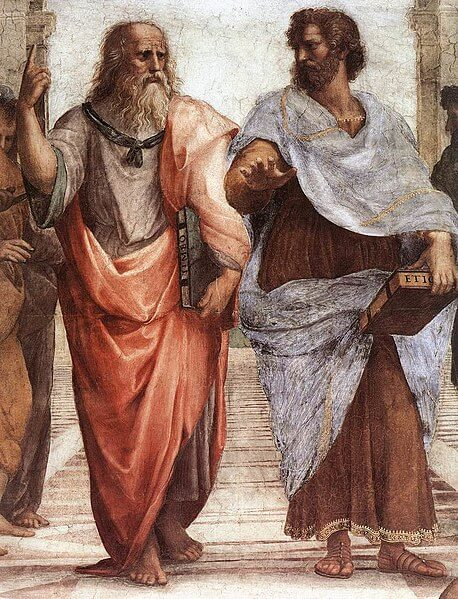
\includegraphics{assets/unit_3/U3_458px-Sanzio_01_Plato_Aristotle.jpg}

\emph{Graphic art of Plato and Aristotle.Photo Credit: \href{https://en.wikipedia.org/wiki/Aristotle\#/media/File:Sanzio_01_Plato_Aristotle.jpg}{Wikipedia}}

\hypertarget{overview-2}{%
\section*{Overview}\label{overview-2}}
\addcontentsline{toc}{section}{Overview}

Welcome to Unit 3!

Suppose you learn that a colleague at work is overcharging for certain items and pocketing the difference? You, being an honest and loyal employee, immediately take him aside and urge him to stop, reminding him that his actions are not only harmful to the company and against policy, but they are simply immoral. To your surprise, your colleague retorts, ``What I'm doing is harmless. The company is big enough that no one will even notice. I agree it's immoral but why should I care about being moral?'' How would you respond to this pointed question?

Have you ever wondered why you or anyone else should care about what is morally good or bad? Is it because you might get caught if you acted immorally, or because others would think less of you? What if you knew you would never get caught? Suppose no one, including God, would ever know if you acted unethically in a certain situation and, thus, no one would ever think less of you or treat you differently. Would you still choose the ethically good action? If so, why?

When we think about ethics, we are usually thinking of how to figure out ethical behaviour. But a deeper question, one that lies behind that question, is why anyone should be moral in the first place.

It is a question we cannot avoid forever because without an answer to it, the entire ethical enterprise is left hanging in the balance. Why put all this effort into trying to figure out what good ethical conduct is if there is no reason to pursue it in the first place? We must come up with some answer but how?

Furthermore, any discussion of the basis of our obligations toward other people immediately presents us with some deeper questions concerning our humanness. These include the following:
- What does it mean to be human?
- More importantly, what does it mean to be a person?
- Are all humans persons by virtue of their humanness?
- Alternatively, do persons have certain characteristics such as self-awareness, the ability to reason, or to carry out self-motivated activity, which certain humans have but others do not at certain stages of development?
- If so, at what point do we become persons with all the rights of personhood? Is it at the point of conception, at birth, or at some point either between these two, or even after the point of birth?

The way we answer these questions will affect our views on such key ethical issues as \textbf{abortion, infanticide, euthanasia, physician-assisted suicide, contraception, in vitro fertilization}, etc. For example, if humans are persons with all the moral rights thereof from conception on, then abortion at any stage of development will be as immoral as ending the life of a three year old child. On the other hand, if humans do not have the rights of personhood until the point of birth, or until some other definite point of development, then abortion, even infanticide, may be morally permissible until they reach that point. Similar reasoning could be applied to the other issues mentioned here.

Rather than focus on these individual issues, in this unit we'll try to
get behind them and explore the basis of our moral obligation. One thing to
remember is that when it comes to answering the question, `Why be moral?' one
answer we cannot give is, ``because it's the right thing to do,'' since, when we
ask, why be moral, we are asking precisely why we should care about doing the
right thing. How, then, can we answer it?

This question has been the subject of intense debate for thousands of years. In this unit, we'll take a short journey down a fascinating trail of case studies, secondary questions, new terms, and different answers to the main question which have been tried out. We'll come across terms like \textbf{Social Contract morality, psychological egoism} and \textbf{ethical egoism}. It is important to understand the meanings of these terms and the different perspectives they bring to our question, ``Why be moral?'' We'll even see if evolutionary biology can help us answer this foundational question about morality. Get ready to read about \textbf{the selfish gene} and \textbf{kin altruism}.

Last, we'll be introduced to the famous story of the Ring of Gyges, told by the ancient Greek philosopher, Plato. It's one of the most intriguing stories of all time relating to the question, why be moral, and it focuses our thoughts on this question. We'll take some time on it in the learning activities for this unit. Once you've read it, it will set the stage for the different answers we'll see to the question.

Let's plunge in. Why be moral?

\hypertarget{topics-2}{%
\subsection*{Topics}\label{topics-2}}
\addcontentsline{toc}{subsection}{Topics}

This unit is divided into 2 topics:

\begin{enumerate}
\def\labelenumi{\arabic{enumi}.}
\tightlist
\item
  Egoism \& Self-interest Morality
\item
  Social Contract Morality
\end{enumerate}

\hypertarget{learning-outcomes-2}{%
\subsection*{Learning Outcomes}\label{learning-outcomes-2}}
\addcontentsline{toc}{subsection}{Learning Outcomes}

When you have completed this unit, you should be able to:
- Explain key ethical concepts such as ethical egoism, psychological egoism,
self-interest morality, and kin altruism.
- Discuss knowledgeably Plato's famous story of the Ring of Gyges.
- Discuss whether people would do what is right, even if no one would find
out.

\hypertarget{activity-checklist-2}{%
\subsection*{Activity Checklist}\label{activity-checklist-2}}
\addcontentsline{toc}{subsection}{Activity Checklist}

Here is a checklist of learning activities you will benefit from in completing
this unit. You may find it useful for planning your work.

\begin{reflect}
\hypertarget{read-view-and-reflect-6}{%
\subsubsection*{Read, View and Reflect}\label{read-view-and-reflect-6}}
\addcontentsline{toc}{subsubsection}{Read, View and Reflect}

Read Chapter 6 on Egoism of your \emph{Introduction} textbook, Wolff, Jonathan. ~\emph{An Introduction to Moral Philosophy}. Watch the video related to the topic.

\hypertarget{wallet-case-study}{%
\subsubsection*{Wallet Case Study}\label{wallet-case-study}}
\addcontentsline{toc}{subsubsection}{Wallet Case Study}

Read and analyze the case study presented.

\hypertarget{read-view-and-reflect-7}{%
\subsubsection*{Read, View and Reflect}\label{read-view-and-reflect-7}}
\addcontentsline{toc}{subsubsection}{Read, View and Reflect}

Read Chapter 7: The Social Contract, in your \emph{Introduction} textbook\emph{.} Watch the videos related to the topic.

\hypertarget{key-terms-quiz-1}{%
\subsubsection*{Key Terms Quiz}\label{key-terms-quiz-1}}
\addcontentsline{toc}{subsubsection}{Key Terms Quiz}

Take the ungraded quiz to review important concepts.

\hypertarget{ethics-committee-response-ungraded}{%
\subsubsection*{Ethics Committee Response (ungraded)}\label{ethics-committee-response-ungraded}}
\addcontentsline{toc}{subsubsection}{Ethics Committee Response (ungraded)}

Meet with your Ethics Committee to discuss the case presented.

\hypertarget{assignment-2}{%
\subsubsection*{\texorpdfstring{\textbf{Assignment}}{Assignment}}\label{assignment-2}}
\addcontentsline{toc}{subsubsection}{\textbf{Assignment}}

Partner Project Presentation (30\%):
This assignment will be presented during weeks 5-10. You must choose a partner and topic this week (see Units 5-10 topics).
\end{reflect}

\hypertarget{resources-2}{%
\subsection*{Resources}\label{resources-2}}
\addcontentsline{toc}{subsection}{Resources}

Here are the resources you will need to complete this unit.
- Wolff, Jonathan. ~\emph{An Introduction to Moral Philosophy}. ~New York: W. W.
Norton \& Company, 2018. ~
- Other online resources will be provided in the unit.

\hypertarget{egoism}{%
\subsection*{Egoism}\label{egoism}}
\addcontentsline{toc}{subsection}{Egoism}

The first topic related to the question, why be moral, comes under the heading of Egoism. There are two kinds of egoism which we will examine, \textbf{psychological egoism} and \textbf{ethical egoism,} and the discussion of these concepts may surprise you. The theories developed around them are similar in certain respects yet give significantly different answers to the question, why be moral.

\textbf{Psychological egoism}, as its name suggests, is a psychological theory about human behaviour and claims that we, humans, cannot help but pursue that which is in our own best interest. It's not difficult to see what this means for our question, why be moral. If this theory is correct, it would make it virtually impossible for anyone to act morally \emph{unless she believed it was in her own best interest to do so}. It will be important to reflect on this theory in the reading to see if it merits our acceptance.

\textbf{Ethical egoism}, as its name indicates, is an ethical theory which teaches
that we have a right, and possibly even a duty, to pursue our own
self-interests. Following our self-interests is the morally right thing to do.

Our text book identifies two distinct forms of ethical egoism. According to one
form, acting in our own self-interest is the best way of advancing the good of
others around us because it is in our self-interest to do good for others. A
society works better when we all look out for the good of others; thus it is in
our best interest to act this way and promote this kind of society.

A different form of ethical egoism, however, holds that it is morally right to act in our own best interests, \emph{regardless of the consequences of others}. The best known proponent of this kind of pure ethical egoism is the Russian-American philosopher and novelist, Ayn Rand, who referred to the ``duty of selfishness.'' We will read briefly about her views in the text reading for this topic.

As we read the chapter on egoism in the Wolff text, think carefully about the
implications this theory, if true, would have for our question, why be moral.

\hypertarget{learning-activities-6}{%
\subsection*{Learning Activities}\label{learning-activities-6}}
\addcontentsline{toc}{subsection}{Learning Activities}

\begin{reflect}
\hypertarget{read-view-and-reflect-8}{%
\subsubsection*{Read, View and Reflect}\label{read-view-and-reflect-8}}
\addcontentsline{toc}{subsubsection}{Read, View and Reflect}

In the first activity, you are asked to read chapters 6 on Egoism of your
textbook, \emph{An Introduction to Moral Philosophy} by Jonathan Wolff. As you read,
be sure to take notes in your Learning Journal, defining key terms and
explaining key concepts. Study the chapter review summary, questions and key
terms. This will help you as you complete the assessments in this course.
Watch the following video that illustrates various types of egoism:

\hypertarget{wallet-case-study-1}{%
\subsubsection*{Wallet Case Study}\label{wallet-case-study-1}}
\addcontentsline{toc}{subsubsection}{Wallet Case Study}

\textbf{Introduction}

Read the following case study and answer the questions in your learning journal.
You are out for a walk in the park when you suddenly spot a wallet lying in the grass. ~Someone has lost it. Upon opening it, you find the I.D. of the owner and contact information; it is someone of whom you have never heard. ~You also find a substantial amount of cash. You have a number of options: leave the wallet alone and continue walking, mail it back to the owner with all its contents inside, or pocket the cash and either mail the wallet back or leave it on the grass. ~If you take the cash, no one will ever know. You think back to your ethics course and realize there are a number of perspectives on your situation.
For this case study, how would a psychological egoist, an ethical egoist, and an advocate of self-interest morality answer the following question: should you pocket the cash? ~Explain why they would each answer as they do.
\end{reflect}

\hypertarget{social-contract-morality}{%
\subsection*{Social Contract Morality}\label{social-contract-morality}}
\addcontentsline{toc}{subsection}{Social Contract Morality}

The second topic related to our question, why be moral, could hardly be more
different from the first. It comes under the heading, Social Contract Morality,
and suggests that moral rules in any society are the result of a social
contract, usually implicit, made between all members of the society. We realize,
say advocates of this theory, that it is in everyone's interests to develop
ethical rules which are to the benefit of all people, and teach them throughout
society. No society could function if everyone did as they wished. Might would
make right, thugs would rule, and life for those who survived would be filled
with fear and exhaustion.

We've seen the difference between the social contract theory and the previous
egoistic ones but can you also see a fundamental similarity between them? This
theory also teaches that the reason we should be moral is that it is in our best
interest to do so. As you read the section in the course text on The Social
Contract, reflect further on this similarity and also on whether it provides an
adequate basis for us to be moral. What problems or questions does it raise?

\hypertarget{learning-activities-7}{%
\subsection*{Learning Activities}\label{learning-activities-7}}
\addcontentsline{toc}{subsection}{Learning Activities}

\begin{reflect}
\hypertarget{read-view-and-reflect-9}{%
\subsubsection*{Read, View and Reflect}\label{read-view-and-reflect-9}}
\addcontentsline{toc}{subsubsection}{Read, View and Reflect}

In this activity, you are asked to read chapter 7, The Social Contract in your
textbook, \emph{An Introduction to Moral Philosophy,} by Jonathan Wolff. Take notes
on key terms and concepts.
Next, watch the following video to get a better understanding of social
contract morality.

\hypertarget{key-terms-quiz-ungraded-2}{%
\subsubsection*{Key Terms Quiz (ungraded)}\label{key-terms-quiz-ungraded-2}}
\addcontentsline{toc}{subsubsection}{Key Terms Quiz (ungraded)}

In order to review some of the major concepts from the text, take the following
unmarked quiz. Although you will not be evaluated on these terms, they will
assist you in the assignments for this course.
Match the following terms to their correct definition.
\end{reflect}

\hypertarget{assessment-2}{%
\subsection*{Assessment}\label{assessment-2}}
\addcontentsline{toc}{subsection}{Assessment}

\begin{assessment}
\hypertarget{assignment-ethics-committee-response-20-1}{%
\subsubsection*{Assignment: Ethics Committee Response (20\%)}\label{assignment-ethics-committee-response-20-1}}
\addcontentsline{toc}{subsubsection}{Assignment: Ethics Committee Response (20\%)}

After completing this unit, including the learning activities, you are asked to
analyze Plato's story of the Ring of Gyges from various perspectives. You will
work again with your Ethics Committee group to discuss the case and then post a
summary report online.

For this Ethics Committee meeting, analyze Plato's story of the Ring of Gyges (from the text reading, p.~88) and state how his key question, ``What would you do?'' might be answered by an ethical egoist, a psychological egoist, an advocate of self-interest morality, and a kin altruist. ~Then explain why you think each would answer as they do. (e.g.~\emph{If I was a \ldots.I would say\ldots{} ~Here is why.)}

As you meet with your Ethics Committee this week, discuss the story and take
notes. In your response, work with key terms and concepts from your readings.
(eg. \emph{If I was a \ldots.I would say\ldots about this case.})

Refer to the \textbf{grading criteria} in the Assessments section of this course.
Submit your report on Moodle by the end of the week.

\hypertarget{assignment-partner-project-presentation-30}{%
\subsubsection*{Assignment: Partner Project Presentation (30\%)}\label{assignment-partner-project-presentation-30}}
\addcontentsline{toc}{subsubsection}{Assignment: Partner Project Presentation (30\%)}

For this partner project, you will choose a specific ethical issue to address.
Please note that this is an argumentative project and not simply a discussion
project. Your presentation should be 12-15 minutes in length and have a visual
element (e.g.~PowerPoint). You will also have an additional 10 minutes at the
end of your presentation to answer questions and facilitate a class discussion.

Note that this assignment will be presented during weeks 5-10. You must choose a partner and topic this week (see Units 5-10 topics). Your Facilitator will hand out a sign-up sheet. Complete this before moving on to the next unit.

See more assignment details, including the \emph{grading criteria} in the Assessments section of this course.

\hypertarget{sign-up-for-the-partner-project-presentation}{%
\subsubsection*{Sign-up for the Partner Project Presentation}\label{sign-up-for-the-partner-project-presentation}}
\addcontentsline{toc}{subsubsection}{Sign-up for the Partner Project Presentation}

For this partner project, your group will choose a specific ethical issue to address.
Please note that this is an argumentative project and not simply a discussion
project. Your presentation should be 12-15 minutes in length and have a visual
element (e.g.~PowerPoint). You will also have an additional 10 minutes at the
end of your presentation to answer questions and facilitate a class discussion.
\end{assessment}

\begin{caution}
\textbf{Note} that this assignment will be presented during weeks 5-10. You must choose a group and topic this week (see Units 3-10 topics). Your Facilitator will hand out a sign-up sheet. Complete this before moving on to the next unit.
\end{caution}

See more assignment details, including the \emph{grading criteria} in the Assessments section of this course.

\hypertarget{checking-your-learning-2}{%
\subsection*{Checking your Learning}\label{checking-your-learning-2}}
\addcontentsline{toc}{subsection}{Checking your Learning}

\begin{progress}
Before you move on to the next unit, you may want to check to make sure that you are able to:
- Explain key ethical concepts such as ethical egoism, psychological egoism, self-interest morality, and kin altruism.
- Discuss knowledgeably Plato's famous story of the Ring of Gyges.
- Discuss whether people would do what is right, even if no one would find out.
\end{progress}

\hypertarget{title}{%
\chapter{Title}\label{title}}

\hypertarget{title-1}{%
\chapter{Title}\label{title-1}}

\hypertarget{title-2}{%
\chapter{Title}\label{title-2}}

\hypertarget{title-3}{%
\chapter{Title}\label{title-3}}

\hypertarget{title-4}{%
\chapter{Title}\label{title-4}}

\hypertarget{references}{%
\chapter*{References}\label{references}}
\addcontentsline{toc}{chapter}{References}

The following are key references used in this course. \textbf{\emph{Check with your course syllabus for required readings.}}

  \bibliography{book.bib}

\end{document}
